\title{Editorial}
\author{por Alessandro Samuel-Rosa}
\maketitle
\begin{wrapfigure}{l}{0.15\textwidth}
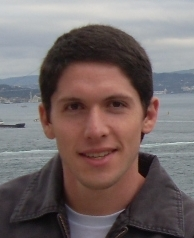
\includegraphics[width=0.15\textwidth]{figuras/foto-alessandro}
\end{wrapfigure}
O segundo número da \textit{Newsletter} da Comissão de Pedometria está cheio de novidades. A principal delas é a nova estrutura, muito mais bonita, graças à inestimável colaboração da comissão editorial do GRASS News, a newsletter do projeto \href{http://grass.osgeo.org/newsletter/}{GRASS}. Após contato com Martin Wegmann \email{wegmann@biozentrum.uni-wuerzburg.de}, editor-chefe do GRASS News, e Dylan Beaudette \email{debeaudette@ucdavis.edu}, administrador da página da web do GRASS News, formos gentilmente autorizados a usar o arquivo de estilo \texttt{GRASSnews.sty}, originalmente derivado do arquivo de estilo \texttt{Rnews.sty}, usado pela equipe do projeto \R{} para produção da sua newsletter. O agora arquivo de estilo da \textit{Newsletter} da Comissão de Pedometria da SBCS, \texttt{PEDOMETRIAnews.sty}, está disponível para baixar \href{http://goo.gl/OBWF3s}{clicando aqui}. É por meio do arquivo de estilo \texttt{PEDOMETRIAnews.sty} que a \textit{Newsletter} fica com a cara que ela tem hoje. Mais informações sobre o uso de \LaTeX{} para a produção de documentos técnico-científicos podem ser encontradas no site da \href{http://www.elsevier.com/author-schemas/preparing-documents-with-tex}{Elsevier}.\\
A evolução da \textit{Newsletter} em seu segundo número acompanha a evolução da pedometria no Brasil, claramente evidenciada pelo volume de trabalhos publicados no Congresso Brasileiro de Ciência do Solo (CBCS), em Florianópolis, há alguns meses atrás. Somam-se aí os espaços destinados mesas de discussão constituídas por importantes pesquisadores da pedometria nacional e internacional. O espaço destinado pela Comissão Organizadora do CBCS mostra que a comunidade científica nacional, assim como já ocorre há mais de uma década em outros países, está muito interessada nas contribuições da mais nova disciplina da ciência do solo. Uma disciplina que exige, como mostram os artigos que seguem, uma abordagem mais do que multidisciplinar ou interdisciplinar. Uma disciplina que exige uma abordagem \href{http://www.fisica-interessante.com/files/artigo-transdisciplinaridade.pdf}{transdisciplinar}, forçando-nos a transpor os limites das disciplinas tradicionais da ciência do solo e mergulhar em um universo de novas maneiras de 
encarar velhos problemas.
%%% Local Variables: 
%%% mode: latex
%%% TeX-master: documento-principal.tex
%%% End: 

